\chapter{Diseño electrónico de un canal de lectura}\label{cap:ro_sch}

\paragraph{}
El canal de lectura es el circuito que lee la información almacenada en los píxeles
tras el tiempo de exposición.
En la arquitectura más habitual, y la que vamos a tratar en este estudio, los
píxeles se leen por columnas, entendiéndose que el chip tiene una dirección
\textit{vertical} y otra \textit{horizontal}. Siguiendo ese criterio, el canal de lectura se
sitúa debajo del array de píxeles de forma que cada columna del canal quede alineada
con cada columna del canal.

\paragraph{}
Idealmente podríamos un canal por columna, y meter en ese espacio todo el circuito
para la columna. Pero, en algunos casos, debido al pequeño tamaño de los píxeles
--- suelen tener unos 5, 8, 10\(\mu m\)... --- resulta complicado o incluso imposible diseñar el
layout de dicha circuitería en ese reducido espacio horizontal. De ahora en adelante
usaremos la palabra inglesa \textit{"pitch''} para referirnos al espaciado con el
que se repite una estructura periódica como el canal de lectura o el array.

\paragraph{}
Por esta razón, es una práctica común usar el \textit{pitch} de varios píxeles, por
ejemplo 2 ó 4, y así tener más espacio para diseñar el layout del circuito. Por contra,
debemos apilar estos 2 ó 4 canales en filas, lo que veremos que nos trae algunos
problemas a la hora de diseñar el layout.

\section{Estructura general}\label{cap:ro_sch_estructura}

\paragraph{}
El canal de lectura es un circuito analógico que va a convertir el voltaje
dado por el pixel tras haber sido expuesto a la luz durante un tiempo y
convertirlo en un valor analógico bien definido entre unos límites que van a
significar \textit{blanco} y \textit{negro}, con una resolución definida.

\paragraph{}
Por tanto, el canal de lectura es principalmente un ADC (en inglés, \textbf{A}nalog
to \textbf{D}igital \textbf{C}onverter, o convertidor analógico-digital).
Una arquitectura usada habitualmente es el convertidor de rampa.
%WARNING
%Ver ventajas del convertidor  de rampa
Éste, para la conversión usa un generador de una rampa de voltaje que se usa para
comparar contra el valor dado por el píxel. Ćuando ambos valores coinciden,
la salida del comparador cambia de estado mediante un flanco de subida o bajada.
De ésta forma la conversión de un valor de tensión se traduce en la detección temporal
de un flanco.

\paragraph{}
De manera simultánea a la rampa analógica se lanza una rampa digital que va contando
valores desde 0 hasta un número que viene determinado por la resolución, y que va a
evolucionar a la misma velocidad que la analógica. Posteriormente, un circuito digital
detectará el flanco y parará el reloj de la cuenta digital, obteniéndose de esta forma
un valor digital para el valor analógico leído.

\section{Operación de lectura}\label{cap:ro_sch_operacion}

\paragraph{}
Para abordar el diseño de un canal de lectura debemos entender como se realiza la
operación de lectura de los píxeles.

\begin{figure}
	\centering
	\begin{subfigure}[b]{0.7\textwidth}
		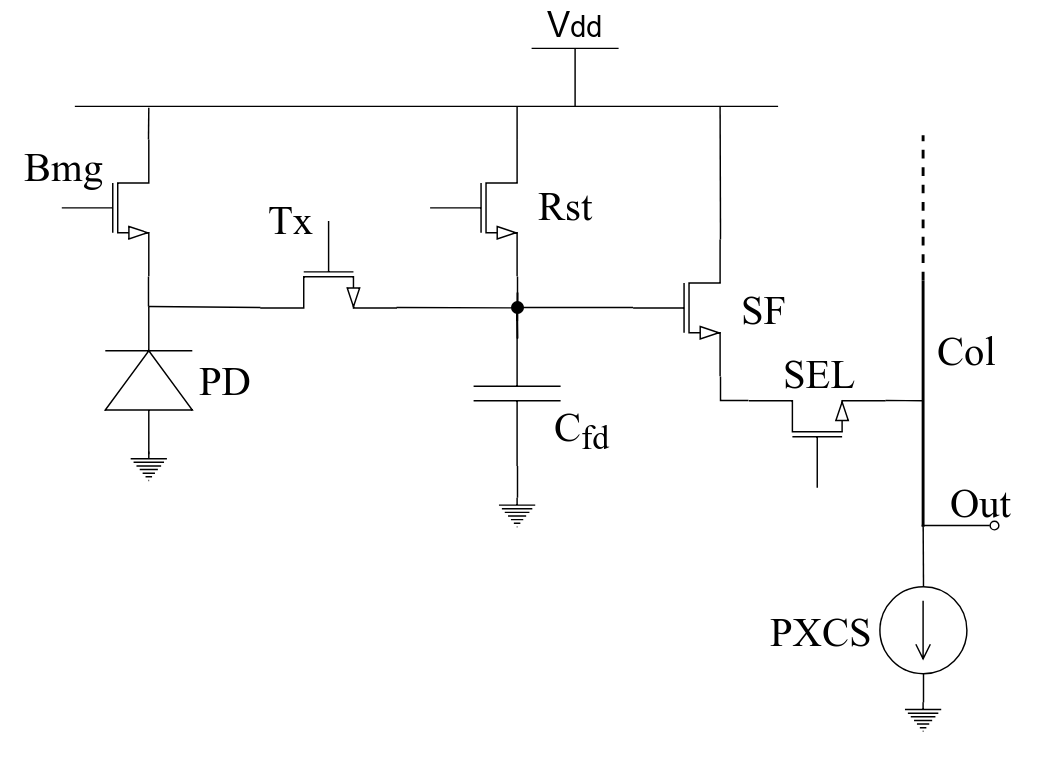
\includegraphics[width=\textwidth]{img/pixel_5T.png}
		\caption{}
		\label{fig:pixel}
	\end{subfigure}

	 %add desired spacing between images, e. g. ~, \quad, \qquad, \hfill etc.
	%(or a blank line to force the subfigure onto a new line)
	\begin{subfigure}[b]{\textwidth}
		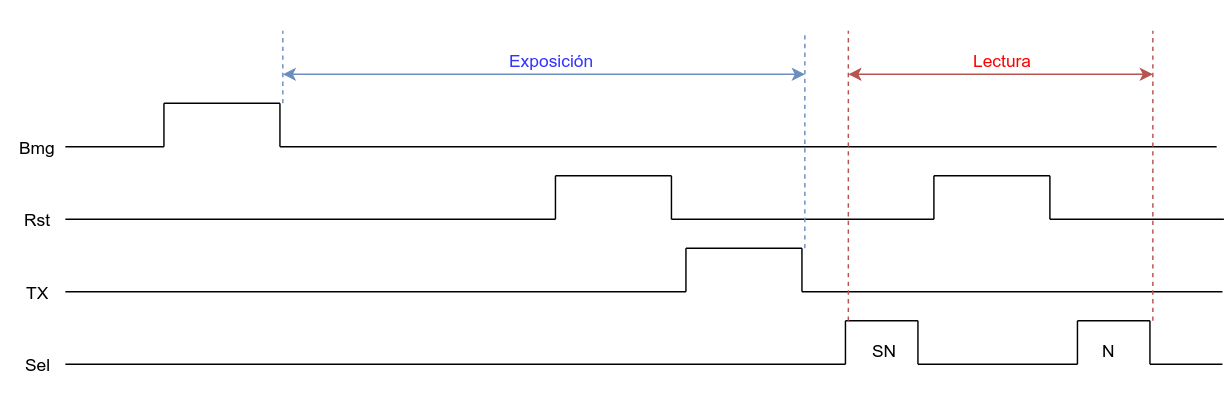
\includegraphics[width=\textwidth]{img/pixel_op.png}
		\caption{}
		\label{fig:pixel_op}
	\end{subfigure}
	\caption{Esquemático y modo operación de un pixel 5T habitual}
	\label{fig:cmos_transistors}
\end{figure}

En la figura \ref{fig:pixel} podemos ver el esquemático de el pixel 5T
que vamos a usar para este estudio. El fotodiodo (PD), es el elemento que más
área ocupa del pixel, ya que es el area que recibe los fotones.

\paragraph{}
Mirando el modo de operación (\ref{fig:pixel_op}) vemos que antes de la exposición se hace un vaciado del
fotodiodo mediante el transistor de BMG, que coloca una tensión alta en el fotodiodo.
Durante la exposición, los electrones fotogenerados van bajando la tensión de este
nodo. Para terminar la exposición, se hace una transferencia de esta carga hacia
el condensador $C_{fd}$ (\textit{Floating Diffusion}), no sin antes dar un pulso
en el transistor de RST (Reset), para vaciar la posible carga que tuviera este condensador.

\paragraph{}
En este punto tenemos la carga con la información de la luz captada por el pixel,
almacenada en el condensador $C_{fd}$, a la espera de que queramos leer este valor
mediante la activación del transistor SEL (Selección). Normalmente, para compensar
errores debidos a asimetrias en los píxeles, se hace una operación de CDS, siglas de
"\textit{Correlated Double Sampling}". Esto es, medir la señal bruta que tenemos
en la "floating diffusion", e inmediatamente después, limpiar este condensador con
un pulso de Reset y volver a leer. De esta forma, simbolizando con S, señal y N,
ruido (\textit{noise}), si restamos ambas formas de onda, podemos obtener:

\begin{equation}
	\label{eq:CDS_operation}
	S = SN - N
\end{equation}

\paragraph{}
Podemos hacer esto debido a que ambas medidas  están correlacionadas porque se
hacen con muy poco tiempo de diferencia y entonces los ruidos son aproximadamente
iguales.

\paragraph{}
Habitualmente existen dos formas de exponer el array: "\textit{global shutter}",
obturación global, y "\textit{rolling shutter}", obturación consecutiva. En la
primera, todas las filas del array se exponen simultáneamente y luego, fila por fila
se van leyendo los valores almacenados en las "\textit{floating diffusions}". En
el segundo caso, la exposición se hace secuencialmente, fila por fila, antes de cada
lectura.

\section{Arquitectura del comparador de rampa}



\section{ADC}



\section{Rampa analógica}

\section{Fuente de corriente}

\section{Bloques de polarización}

\section{Rampa digital y serialización}
